
\chapter{Related Work}
\label{ch:realted_work}

This chapter will give a brief introduction to neural networks and time delay neural networks, as well as an introduction automated speech recognition with hidden markov models. These are the necessary building blocks for the work presented in this thesis. At the end of this chapter, we will also briefly present research that directly inspired this work. 

\section{Neural Networks}
\label{sec:neural_networks}

In machine learning research, the goal of a \textit{neural network} is to approximate arbitrary functions. The basic idea of neural networks, so called \textit{perceptrons}, were first introduced by Rosenblatt in \cite{rosenblatt1958perceptron}. While the first neural networks were biologically motivated, neural networks can be interpreted as composition of functions. The relation between these functions forms a directed graph. In this work, we will only cover \textit{feed forward neural networks}. They are called feed forward neural networks because there are no feedback connections: The relation between all functions in the neural network forms an acyclic directed graph. Feed forward networks are an important building block for many machine learning applications. 
\\
More formally, as described in \cite{Goodfellow-et-al-2016}, a feed forward neural network can be described as a model $y = f^*(x, \theta)$, approximating an existing function $y = f(x)$. In this example $x$ is the input, $y$ is the output and $\theta$ are the model parameters which are learned during training. $f$ is the function to approximate and $f^*$ is a composition of many functions with the parameters $\theta$. 
\\
In practice, the functions composing a feed forward neural network are often simply chained, so that their relation graph simply forms a path. In this case, the functional components are called layers. A feed forward neural network of this form with $n$ layers can be written as follows:

\[
y = f^*_n \dots (f^*_2(f^*_1(x, \theta_1), \theta_2) \dots, \theta_n)
\]

For this type of neural network, $f^*_1$ is applied to the input, then $f^*_2$ is applied to the output of $f^*_1$, until the final layer is reached. The output of the final layer is the output of the neural network. Figure \ref{fig:simple_feed_forward_nn} shows a graph based representation of such a neural network. Each node represents a function, arrows represent data flows. 

\begin{minipage}{\linewidth}
	\makebox[\linewidth]{
	\begin{tikzpicture}[x=1.5cm, y=1.5cm, >=stealth]
	
	\node [every neuron] (n0) at (0*1-1,2.5-0) {$x$}; 
	\node [every neuron] (n1) at (1*1-1,2.5-0) {$f^*_1$}; 
	\node [every neuron] (n2) at (2*1-1,2.5-0) {$f^*_2$}; 
	\node [neuron hmissing] (n3) at (3*1-1,2.5-0) {}; 
	\node [every neuron] (n4) at (4*1-1,2.5-0) {$f^*_n$}; 
	\node [every neuron] (n5) at (5*1-1,2.5-0) {$y$}; 
	
	\draw [->] (n0) -- (n1);
	\draw [->] (n1) -- (n2);
	\draw [->] (n2) -- (n3);
	\draw [->] (n3) -- (n4);
	\draw [->] (n4) -- (n5);
	
	\end{tikzpicture}
	}
	\captionof{figure}{Simple graphical interpretation of feed forward neural network}
	\label{fig:simple_feed_forward_nn}
	\hspace{1cm}
\end{minipage}


Even with this simplification, it has been shown that such a feed forward neural network can approximate any function with any desired accuracy. This is called the \textit{universal approximation theorem}, the proof can be found in \cite{hornik1989multilayer}. The caveat is finding the correct function $f^*_n$ to use in each layer and the correct parameters $\theta_n$. Also, finding the function to approximate is non-trivial in the first place. We will discuss these problems in the next sections. 

\subsection{Training Neural Networks}

As with most machine learning approaches, we train the neural  network using by using a \textit{training dataset}, containing a lot of data points sampled from the distribution we seek to approximate. We usually do not want the neural network to excel on the training data set, but rather to perform well on unseen data. This ability is called \textit{generalization}. We can approximate the error on unseen data by testing the neural network on a \textit{test dataset}. The test dataset must never be used for adjusting the neural network parameters, as this will make the test dataset worthless. The situation where a network performs well on the training dataset but worse on the test dataset is called \textit{overfitting}. The network basically memorizes the distribution of the training dataset, but fails to generalize on the test dataset. \\
Given the definition in the past section, we can treat the problem of training a given neural network as finding appropriate parameters $\theta$ to minimize a certain \textit{error function} or \textit{loss function} $E = \mathcal{L}(y)$, where $E$ denotes the error and $y$ the network output. The error $E$ is usually some metric that judges the network performance based on the training data set. The state of the art algorithm for optimizing the parameters of a neural network is called \textit{stochastic gradient descend}, a special application of naive \textit{gradient descend}.
\subsubsection{Naive Gradient Descent}
\label{sec:gradient_descend}
To apply gradient descend, we have to calculate the derivative of the loss function, given a certain input, with respect to a certain parameter $\theta_i$. Since this derivative is multi-dimensional, it is called the \textit{gradient}. Given a feed forward neural network, we can write the error as follows:

\[
E = \mathcal{L}(f^*_n \dots (f^*_2(f^*_1(x, \theta_1), \theta_2) \dots, \theta_n))
\]

Thus, the derivative of the error with respect to a certain weight can be calculated by applying the chain rule.  

\[
\frac{\delta E}{\delta \theta_i} = 
	\frac{\delta \mathcal{L}}{\delta y_n}
	\frac{\delta f^*_n}{\delta y_{n - 1}}
	\dots
	\frac{\delta f^*_{i + 2}}{\delta y_i}
	\frac{\delta f^*_i}{\delta \theta_i}
\]

Where $y_k$ is the result of $f^*_k$. \\
We know that the gradient $\frac{\delta E}{\delta \theta_i}$ will become zero in a local minimum, local maximum or saddle point of our error $E$. Since the gradient also gives the direction of the steepest slope, we can simply update our parameters iteratively, until we converge into a local minimum.

\[
	\theta_{i, t+1} = \theta_{i, t} - \epsilon * \frac{\delta E_{t}}{\delta \theta_{i, t}}
\]

In this equation, $t$ denotes the current time and the parameter $\epsilon$ is the so-called learning rate. $\epsilon$ has to be chosen by the designer of the neural network and influences not only the speed of convergence, but also whether the network converges at all. In literature, propagating the error gradient through a neural network is called \textit{backpropagation}. Backpropagation in the context of neural networks was first described in \cite{werbos1974beyond}.

\subsubsection{Stochastic Gradient Descend}

In practice, naive gradient descend does not work well, as described in \cite{wilson2003general}. The reason is that the function we seek to optimize when training a neural network is not convex and might have many local minima. Optimizing iteratively on a stationary error term makes this approach prone to falling into local minima. \\ \\
The state of the art algorithm for training neural networks is called \textit{stochastic gradient descent} (\textit{SGD}), which was first described in a context of neural networks in \cite{bottou1991stochastic}. Stochastic gradient descent introduces two fundamental changes and is. First, we no longer calculate our error term and corresponding gradient for the whole dataset, but for a randomly sampled subset of our data set, which is called a \textit{mini batch}, where the size of the mini batches is a design parameter. Second, we decrease our learning rate while training progresses. According to \cite{Goodfellow-et-al-2016}, iterating on mini batches adds noise to our error term, which in turn offers a regularization effect which was shown to lead to better generalization.
\\ \\
The noise introduced by stochastic gradient descend originates from the fact that we batch our dataset. Even if all batches, if averaged, represent the same distribution as our whole test dataset, each batch has a slightly different distribution. The shape of the loss function, and thus the gradient, changes slightly with each mini batch. This is the main reason why stochastic gradient descend is less prone to get stuck in local minima then naive gradient descend. The noise added by this stochastic process does not go away, even when we reach a global minimum. According to \cite{Goodfellow-et-al-2016}, this is be the main motivation for decreasing the learning rate over time. Furthermore, this property implies that the mini batch size is also an important design choice for achieving good generalization, not only for achieving fast training. 
\\ \\
A disadvantage of stochastic gradient descend is the slower convergence, since we need more steps. This is remedied by the fact that it is easier to calculate the gradient for a small mini batch instead of the whole dataset at once. In practice, we usually shuffle our dataset, split it into mini-batches, and then process each mini batch once. An iteration over all mini batches in the dataset is called an \textit{epoch}. 

\subsubsection{Learning Rates and Learning Rate Scheduling}

With stochastic gradient descend, we choose a separate learning rate $\epsilon_k$ for each epoch $k$. In the scope of this work, we only introduce \textit{exponential decay}, a very simple scheduling algorithm for the learning rate, although numerous other schedulers exist. \\
Exponential starts with a learning rate $k_0$ for the initial batch and multiplies the learning rate by a factor of $0 < p < 1$ after each epoch. 
\[
k_n = k_{n - 1} * p
\]
A variant of exponential decay keeps the learning rate constant for a number epochs, until the improvement of error measured on the test dataset falls below a certain threshold $t$. This variant is called \textit{newbob}. Newbob scheduling is widely used by the speech recognition community. It was first introduced in \cite{berkely2000newbob}.

\subsubsection{Momentum}

\textit{Momentum} is another technique that was shown to avoid local minima. When using momentum, we do not apply the gradient directly to our model, but rather use a linear combination of the gradient of the last batches. There are multiple versions to achieve momentum when using stochastic gradient descend. This work uses the notation introduced in \ref{polyak1964some} and throughly analyzed in the context of deep learning in \ref{sutskever2013importance}:
\begin{align*}
\upsilon_{i, t+1} &= \upsilon_{i, t} * \rho + \epsilon * \frac{\delta E_{t}}{\delta \theta_{i, t}} \\
\theta_{i, t+1} &= \theta_{i, t} - \upsilon_{i, t+1}
\end{align*}
Here, $\upsilon$ is called the \textit{velocity}, it is a linear combination of the last velocity and the current gradient. $\rho$ is the term defining the momentum. It defines how much of the velocity is added to the current gradient. All other variables are defined as in section \ref{sec:gradient_descend}.

\subsection{Neural Network Architectures}

In practice, neural network layers are often formed by combining an affine transformation with a non-linear function. Since affine transformations of data vectors can be interpreted as matrix-vector multiplications, we can write a layer function in the following way, where $x_k$ is the input vector for $k$th layer, $W_k$ is the matrix defining the affine transformation of the $k$th layer, and $\varphi$ is a non-linear activation function of layer $k$.
\[
f^*_k(x_k) = \varphi_k(W_k x_k)  
\]
The count of layers, as well as the size of each $W_k$ are design decisions and depend on the task. We call the count of layers \textit{depth} of a neural network, and count of rows in $W_k$ the \textit{width} of layer $k$. The contents of $W_k$, called the \textit{weights} of layer $k$, are the trainable parameters $\theta$ for models of this form.
\pagebreak
\subsubsection{Activation Functions}

Non-linear activation functions, or simply \textit{activation functions}, can be roughly classified into two groups: Activation functions which are applied element-wise and thus do not change the dimension of the data, as well as activation functions which are applied on groups of elements of the input vector and change the dimension. The latter case is commonly fund with so called pooling functions. The choice of the activation function $\varphi$ has significant impact on the performance of a neural network and has been subject to many bodies of research, as summarized in \cite{thoma2017analysis}. In this work, we will only discuss the \textit{ReLU}, \textit{p-norm} and \textit{softmax} activation functions. 

\subsubsection*{Rectified Linear Unit (ReLU)}
% ReLU
\begin{minipage}{0.45\textwidth}
	\[\varphi^{ReLU}(x) = \begin{cases}
	0 & x < 0 \\
	x & x \geq 0
	\end{cases}\]
	First introduced in \cite{krizhevsky2012imagenet}, ReLU nonlinearities have proven successful in practice. The computation of ReLU nonlinearity is cheap, also the gradient never saturates for positive values of $x$. For negative values, the gradient is zero, which can be a disadvantage.  
\end{minipage}
\hfill
\begin{minipage}{0.45\textwidth}
\begin{tikzpicture}[baseline=(current bounding box)]
\begin{axis}[xmin=-2,xmax=2,ymin=-2,ymax=2,axis lines = middle,xlabel = $x$,ylabel = $\varphi^{ReLu}(x)$,clip = false]
\addplot+[mark=none,blue,domain=-2:0] {0};
\addplot+[mark=none,blue,domain=0:2] {x};
\end{axis}
\end{tikzpicture} 
\captionof{figure}{The ReLU function.}
\end{minipage}
% L2 Pooling

\subsubsection*{P-norm}
\begin{minipage}{0.45\textwidth}
	\[\varphi^{Lp}(X) = \sqrt[p]{ \sum_{x \in X}{x^p} } \] 
	The p-norm nonlinearity was described by \cite{zhang2014improving}. This nonlinearity operates on a set $X$ of input elements and reduces them to one. The group size as well as the $p$ are a design parameter. For a fixed $p$ of $2$, the p-norm is also called \text{L2 pooling}.
\end{minipage}
\hfill
\begin{minipage}{0.45\textwidth}
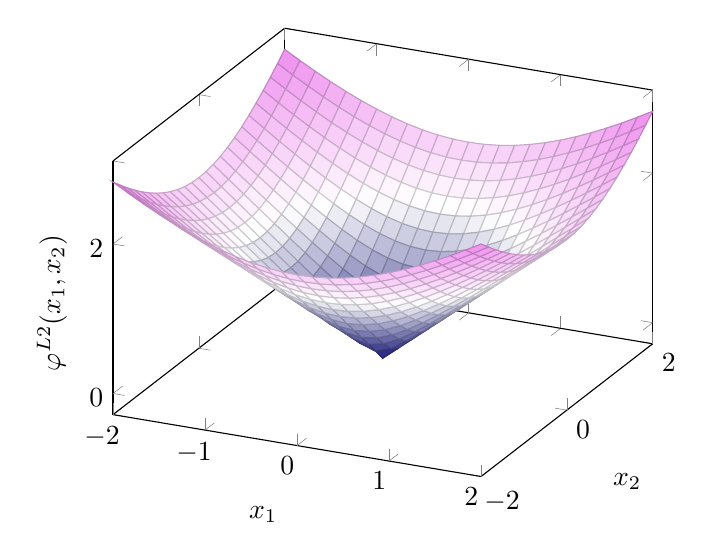
\begin{tikzpicture}[baseline=(current bounding box)]
\begin{axis}[xmin=-2,xmax=2,ymin=-2,ymax=2,xlabel = $x_1$,ylabel = $x_2$,zlabel = $\varphi^{L2}({x_1, x_2})$,colormap/violet,clip = false]
\addplot3[surf,samples=25, domain=-2:2]
{sqrt(x * x + y * y)};
\end{axis}
\end{tikzpicture}
\captionof{figure}{Example of p-norm with $p = 2$ and and an input group containing two values}
\end{minipage}

\subsubsection*{Softmax}
\begin{minipage}{0.45\textwidth}
	\[\varphi^{softmax}_{\tau}(X)_i = \frac{e^\frac{x_i}{\tau}}{ \sum_{x_j \in X} e^\frac{x_j}{\tau} } \]
	The softmax activation is defined as an operation over the whole input, but does not reduce the dimension. It maps all output values to a space between $0$ and $1$, preserves the rank of each output and also guarantees that the sum over all outputs is exactly $1$. Therefore it produces a valid probability distribution and is usually used for the last layer of a neural network for classification problems. The term $\tau$ is called the softmax temperature. It can be used to change the contrast of the distribution produced by the softmax activation. A higher temperature $\tau$ will lead to a distribution more smooth. A lower $\tau$ will lead to a more sharp distribution, that concentrates a higher probability at the maximum value. 
\end{minipage}
\hfill
\begin{minipage}{0.45\textwidth}
	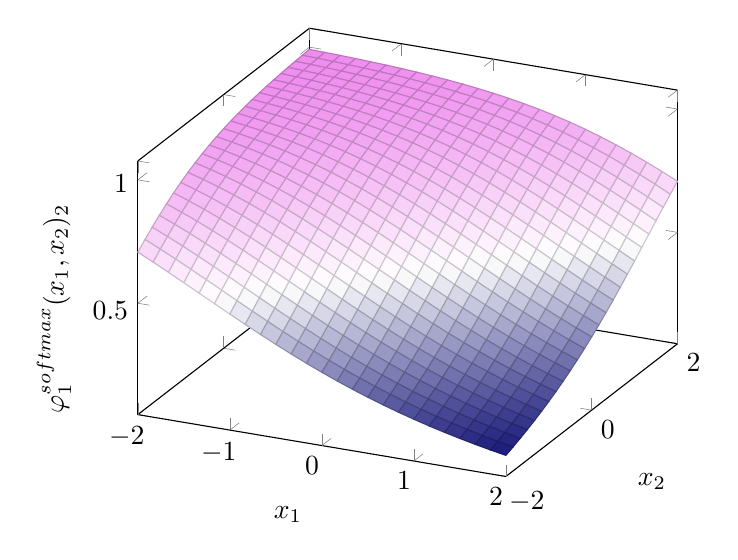
\begin{tikzpicture}[baseline=(current bounding box)]
	\begin{axis}[xmin=-2,xmax=2,ymin=-2,ymax=2,xlabel = $x_1$,ylabel = $x_2$,zlabel = $\varphi^{softmax}_{1}({x_1, x_2})_2$,colormap/violet,clip = false]
	\addplot3[surf,samples=25, domain=-2:2]
	{sqrt(e^y / (e^x + e^y) )};
	\end{axis}
	\end{tikzpicture}
	\captionof{figure}{Example of a vanilla softmax ($\tau = 1$) for an input vector containing two values}
	\vspace{0.5cm}
	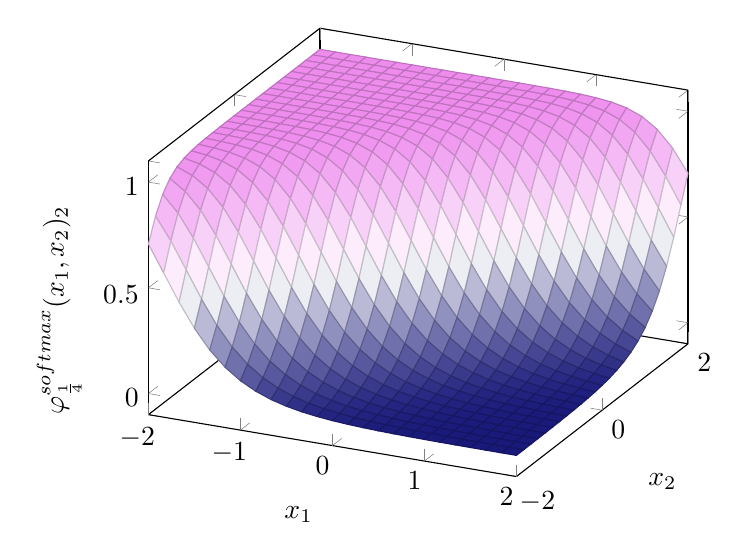
\begin{tikzpicture}[baseline=(current bounding box)]
	\begin{axis}[xmin=-2,xmax=2,ymin=-2,ymax=2,xlabel = $x_1$,ylabel = $x_2$,zlabel = $\varphi^{softmax}_{\frac{1}{4}}({x_1, x_2})_2$,colormap/violet,clip = false]
	\addplot3[surf,samples=25, domain=-2:2]
	{sqrt(e^(y * 4) / (e^(x * 4) + e^(y * 4)) )};
	\end{axis}
	\end{tikzpicture}
	\captionof{figure}{Example of a softmax with adjusted temperature ($\tau = \frac{1}{4}$) for an input vector containing two values}
\end{minipage}

\subsection{The Cross Entropy Loss Function}

There exist numerous loss functions for neural networks. Technically, any metric can be used as loss function, although loss functions do not necessarily have to be metrics. One of the most widely loss functions for classification tasks is the \textit{cross entropy} (\textit{CE}) function. For two  probability vectors $p$ and $q$, the cross entropy can be written as follows:

\begin{align}
H(p, q) = - \sum_{x} p(x) \log q(x)
\label{eq:cross_entropy_loss}
\end{align}

The cross entropy loss function has several important properties. First, it minimizes the so called \textit{Kullback-Leibler} (\textit{KL}) divergence. The Kullback-Leibler divergence measures the distance of two probability distributions and was introduced in \cite{kullback1951information}. The Kullback-Leibler divergence is equal to zero if, and only if, the two given distributions are also equal. For two probability vectors $p$ and $q$, it can be written in the following way:

\[
D_{KL}(p, q) = -\sum_{x} p(x) \log \frac{p(x)}{q(x)}
\]

To show the connection between the cross entropy and the Kullback-Leibler divergence, we first assume that $q$ is the distribution we seek to optimize. Thus $p$ can be thought of as an example from our training dataset, or in other words, the distribution we seek to match. Therefore, $p$, can be assumed to be constant. We can write the Kullback-Leibler divergence as follows: 

\begin{align*}
D_{KL}(p, q) &= - \sum_{x} p(x) \left[ \log p(x) - \log q(x) \right] \\
& = - \sum_{x} p(x) \log p(x) -\sum_{x} p(x) \log q(x)
\end{align*}

Since we are not interested minimizing the distribution $p$, we can drop the first sum, and thus receive the cross entropy loss as in equation \ref{eq:cross_entropy_loss}. \\ \\
When training neural networks, we often deal with classification problems. In this case, we seek to assign a single class to a given input sample, our target probability $p$ has exactly one element which is one, all other elements are zero. In this case, the cross entropy loss can be simplified to the so called \textit{negative log likelihood loss}, where $i$ is the index of the correct class in $p$. 

\[
D_{NLLL}(i, q) = -\log q(i)
\]

It has to be noted that this loss functions all operate on probability vectors: All elements have to be between $0$ and $1$ and sum to unity. Therefore, a softmax activation function is usually applied before calculating the loss. 

TODO: Section about practical considerations, like data augmentation? 

\section{Automated Speech Recognition}
\label{ch:HMM_ASR}
\textit{Automated speech recognition} (\textit{ASR}) is the task of generating a text transcription from a given sample of spoken language using a computer system. In literature, this problem is also referred to as \textit{speech to text} (\textit{SST}). \\
Many approaches exist for solving this task. In this work, we will focus on automated speech recognition using systems that are based on hidden markov models for modeling language. The contents of this this section, except otherwise noted, is based upon the lecture Automated Speech Recognition of Karlsruhe Institute of Technology \cite{kitasr2018stueker}, which is in turn based on the books \cite{schukat1995automatische} and \cite{huang2001spoken}. \\ \\
Automated speech recognition systems built on hidden markov models usually follows an architecture that separates \textit{preprocessing} of the audio signal and \textit{decoding}. The preprocessing transforms a brief time window of the audio signal into a feature vector. The decoding uses a statistical model assembled from an \textit{acoustic model}, a \textit{dictionary} and a \textit{language model} to calculate the most likely text representation, given the feature vectors.\\ \\

More formally, we can treat the decoding as a classification problem. Let $a$ be a set of feature vectors, we seek to find the word sequence $w^*$ that was most likely for $a$ under our model. That can formally be written as follows, where $p(w|a)$ is the conditional probability of event $w$ given $a$:

\[
w^* = \underset{w}{\arg \max} \; P(w|a)
\] 
We do not know $P(w|a)$, but can re-write it using Bayes' theorem:

\[
w^* = \underset{w}{\arg \max} \; \frac{P(a|w) P(w)}{P(a)}
\]

Since $p(a)$ is the same for all possible word sequences $w$, we can drop the denominator from this equation:

\begin{align}
w^* = \underset{w}{\arg \max} \; P(a|w) P(w)
\label{eq:asr_base_formula}
\end{align}

Equation \ref{eq:asr_base_formula} is called the \textit{fundamental equation of automated speech recognition}. While the fundamental equation seems straight forward, the difficult task is to create a reliable and computationally tractable model for approximating the probability of an acoustic feature given a word sequence, $p(a|w)$ and the probability of observing a word sequence $p(w)$. For this task, \textit{hidden markov models} built from the acoustic model, language model and dictionary are used. We will first describe the preprocessing, then briefly introduce hidden markov models, then introduce the three components and then show how they are combined into a single model, which is then used by the decoder. 

\subsection{Preprocessing}
Preprocessing transforms some audio signal into a sequence of feature vectors. To do so, we sample an audio signal using a microphone, then the signal is windowed and the spectrum is calculated for each window of the signal. This process is called short time fourier transform, as defined in the introduction in equation \ref{eq:stft}. Hence, the resulting spectral coefficients are also often called \textit{fourier coefficients}. It should be noted that there are more sophisticated approaches, notably the \textit{continous wavelet transform}, as described in \cite{mallat1999wavelet}, which has better properties in terms of time and frequency resolution. \\ \\
There exist numerous approaches to transform the spectrum of a signal to useful features. In this work, we only discuss so called \textit{log-mel coefficients}. 
\subsubsection{Log-Mel Coefficients}
Log-mel coefficients were introduced in \cite{waibel1990phoneme} and \cite{waibel1983comparative}. This approach is physiologically motivated. To be specific, the mel-scale provides a better relative frequency resolution in lower frequencies. \\
As given in \cite{poser1990speech}, the mel-scale is defined by the following relation to the regular frequency spectrum in Hertz: 
\[
MEL(f)=2595\log _{10}\left(1+{\frac {f}{700}}\right)
\]
Very often, the number of coefficients is reduced to get smaller feature vectors $(\sigma_1, ..., \sigma_n)$. This is done by summing all coefficients in certain windows $\sigma_k$ on the mel-scale: 
\[
MEL_k = \int \sigma_k(f) * MEL(f) \delta f 
\]

In practice, a triangle window is often used. \\
The $k$-th log-mel coefficient is then calculated by applying a logarithm:
\[
lMEL_k = \log(MEL_k) 
\]
\\ \\
In literature, \textit{Mel-Frequency-Cepstral-Coefficients} (\textit{MFCCs}) are often mentioned. They are not to be confused with log-mel coefficients. MFCCs can be calculated by applying an inverse discrete cosine transform on the the log-mel coefficients.

\subsubsection{Vocal Tract Length Normalization}
TODO: 
https://www.lti.cs.cmu.edu/sites/default/files/CMU-LTI-97-150-T.pdf

\subsection{Hidden Markov Models}
To explain hidden markov models, we first introduce the concept of a \textit{markov chain}. A markov chain is a sequence of random variables $X = x_1, x_2, \dots. x_{t - 1}, x_{t} \dots, x_T$ and a finite number of states $s_1, \dots, s_n$, where the probability of each entering a certain state at time $t + 1$ at only depends on the state at time $t$:

\[
P(x_{t + 1} = s_{j_{t + 1}} | x_{t} = s_{j_t}, x_{t - 1} = s_{j_{t - 1}} \dots, x_{1} = s_{j_{1}}) = P(x_{t + 1} = s_{j_{t + 1}} | x_{t} = s_{j_t})
\] 

This assumption is also called the \textit{markov assumption}. If the probability of moving from state $s_{j_t}$ to state $s_{j_{t + 1}}$ is independent of the current time $t$, we call a markov chain \textit{homogeneous}. \\ \\
We now extend our homogeneous markov chain and assume that we can no longer observe the state $s_{j_t}$ at a given time $t$ directly, but a symbol $v_k$ that was emitted. We formally define: 
\begin{align*}
S &= \{s_1, \dots, s_n\} \tag{states} \\
V &= \{v_1, \dots, v_m\} \tag{symbols} \\
A &= (a_{ij}) \tag{state tansmission probability} \\
a_{ij} &= p(x_{t+1} = s_j | x_{t} = s_i) \\
B(k) &= (b_j(k)) \tag{emisson probability} \\
b_j(k) &= p(v_k | x_t = s_j) \\
\pi &= (\pi_i) \tag{initial state probability} \\
\pi_i &= p(x_1 = s_i)
\end{align*}

The tuple $\lambda = (S, V, A, B, \pi)$ specifies a \textit{hidden markov model}. We furthermore introduce the graphical notation for hidden markov models seen in figure \ref{fig:hmm}. Unspecified transitions and observations have probability zero. 

\begin{minipage}{\linewidth}
	\makebox[\linewidth]{
		\begin{tikzpicture}[x=1.5cm, y=1.5cm, >=stealth]
		
		\node[state] (s1) at (0,2) {$s_1$}
		edge [loop above] node[above] {$a_{11}$} ();
		\node[state] (s2) at (3,2) {$s_2$}
		edge [<-,bend right=45] node[auto,swap] {$a_{12}$} (s1)
		edge [->,bend left=45] node[auto,swap] {$a_{21}$} (s1)
		edge [loop above] node[above] {$a_{22}$} ();
		\node[state] (s3) at (6,2) {$s_3$}
		edge [<-,bend right=45] node[auto,swap] {$a_{23}$} (s2)
		edge [->,bend left=45] node[auto,swap] {$a_{32}$} (s2)
		edge [loop above] node[above] {$a_{33}$} ();
		% observations
		\node[observation] (v1) at (1.5,0) {$v_1$}
		edge [lightedge] node[auto] {$b_1(1)$} (s1)
		edge [lightedge] node[auto,swap] {$b_2(1)$} (s2);
		\node[observation] (v2) at (4.5,0) {$v_2$}
		edge [lightedge] node[auto] {$b_2(2)$} (s2)
		edge [lightedge] node[auto,swap] {$b_3(2)$} (s3);
		\end{tikzpicture}
	}
	\captionof{figure}{Graphical example of a hidden markov model with three states and two observations}
	\label{fig:hmm}
	\hspace{1cm}
\end{minipage}

\subsubsection{Forward and Backward algorithm}
Given a sequence of observed emissions, a so called observation $O = \{o_1, \dots, o_t\}$, a hidden markov model can be used to evaluate the probability of the observation, given the parameters $p(O, \lambda)$. For calculating this joint probability, the \textit{forward algorithm} or the \textit{backward algorithm} can be used used. For the forward algorithm, let $\alpha_T(j)$ be the probability of having observed $O$ and being in state $s_j$ at the end of the observation. We define recursively for any previous time $t$:
\begin{align*}
\alpha_1(j) &= \pi_j b_j(o_1) \\
\alpha_t(j) &= b_j \sum_{i = 1}^{N} a_{ij}\alpha_{t-1}(i) \\
p(O|\lambda) &= \sum_{j = 1}^{N} \alpha_T(j)
\end{align*}
For the backward algorithm, we define a similar recursive algorithm, starting from the latest time observation. Here, $\beta_0(j)$ is the probability of observing $O$ when starting from state $s_j$.
\begin{align*}
\beta_T(j) &= 1 \\
\beta_t(j) &= \sum_{i = 1}^{N} a_{ij}b_j(o_{t+1}) \beta_{t+1}(i) \\
p(O|\lambda) &= \sum_{j = 1}^{N} \beta_0(j)
\end{align*}
\subsubsection{Decoding Problem}
Besides calculating the probability of an observation sequence, finding the most likely state sequence $X = \{X_1, X_2, \dots, X_T\}$ given an observation $O$ and a hidden markov model $\lambda$ is also of interest. 
This problem is called the \textit{decoding problem}, which is solved by the \textit{viterbi algorithm}. In the scope of this work, a formal definition of the viterbi algorithm is not necessary. 

\subsubsection{Learning Hidden Markov Model Parameters}
Given a hidden markov model topology, which is essentially only the number of states $n$ and the number of emission symbols $m$, as well as a training set of observations $O$, we can use the so called \textit{Baum-Welch} algorithm to optimize the initial state probabilities $\pi$, transmission probabilities $A$ and emission probabilities $B$. \\ \\
We first define two auxiliary variables, given an observation $O$ and the parameters $\lambda$: $\gamma_t(i)$, the probability of being in state $i$ at time $t$ and $\xi_t(i, j)$, the probability of being $i$ at time $t$ and state $j$ at time $t + 1$.

\begin{minipage}{0.45\textwidth}
\begin{align*}
\gamma_t(i) &= P(x_t = i|O,\lambda) \\
&= \frac{P(x_t = i, O|\lambda)}{P(O|\lambda)} \\
&=\frac{\alpha_t(i)\beta_t(i)}{\sum_{j = 1}^{N} \alpha_t(j) \beta_t(j)} 
\end{align*}
\end{minipage}
\hfill
\begin{minipage}{0.45\textwidth}
\begin{align*}
\xi_t(i, j) &= P(x_t = i,x_{t + 1} = j|O,\lambda) \\
&= \frac{P(x_t = i,x_{t + 1} = j, O|\lambda)}{P(O|\lambda)} \\
&=\frac{\alpha_t(i)a_{ij}\beta_{t + 1}(j)b_j(o_{t + 1})}{\sum_{i = 1}^{N} \sum_{j = 1}^{N} \alpha_t(i)a_{ij}\beta_{t + 1}(j)b_j(o_{t + 1})}
\end{align*}
\end{minipage}

Using this two auxiliary variables, we can find new parameters $\lambda$ iteratively. Let $\pi^*$, $A^*$ and $B^*$ be the new parameters after one iteration of the Baum-Welch algorithm. 

\begin{align*}
b^*_j(k) &= \frac{\sum_{t = 1, o_t = v_k}^{T} \gamma_t(j)}{\sum_{t = 1}^{T} \gamma_t(j)} \\
\pi^*_i &= \gamma_1(i) \\
a_{ij}^*  &= \frac{\sum_{t = 1}^{T} \xi_t(i, j)}{\sum_{t = 1}^{T} \gamma_t(j)} 
\end{align*}

It should be noted that the Baum-Welch algorithm is a special case of the \textit{expected maximization} {\textit{EM}} algorithm applied to hidden markov models. The expected maximization algorithm gives a maximum-likelihood estimate of parameters, even if the data set used for the estimation has incomplete or missing values. A proof can be found in \cite{bilmes1998gentle}. 

\subsection{Acoustic Model}
\label{sec:acoustic_model}
Before we explain the purpose of the acoustic model, we have to introduce the linguistic concepts of \textit{phonemes}, \textit{phones} and \textit{allophones}. Phonemes are sound atoms in a spoken language, that are relevant for the meaning of a spoken word. In other words, if a phoneme in a spoken word changes, the meaning of this word would change. Allophones are different pronunciation version of the same phoneme. \textit{Phones} are simply distinct sounds that are found in a language, regardless of whether swapping a phone changes the meaning of the word or not. \\ \\
The acoustic model $A$ is responsible of giving us the probability of observing a certain feature $o$, for a given phone $\wp$. 
\[
	A_\wp(o) = p(o|\wp)
\]
Traditional acoustic models use classification schemes on feature vectors from the preprocessing. The most prominent technique here are gaussian mixture models, which combine several normal distributions to approximate a more complex distribution. The parameters of the acoustic model are usually learned using the Baum-Welch equations introduced in the previous section. \\ \\
Acoustic models might be extended to classifying allophones, or even include context dependencies on neighboring phones. Antother approach would be to model the start, middle, and end part of an phone as three distinct hidden markov model states, which represent the phone together. This has the advantage of introducing some speed invariance into the model: It does no longer matter whether a certain phoneme was spoken very slowly or fast. Figure \ref{fig:sub_three_allophone} shows a hidden markov model for such an approach. 

\begin{minipage}{\linewidth}
	\makebox[\linewidth]{
		\begin{tikzpicture}[x=1.5cm, y=1.5cm, >=stealth]
		
		\node[state] (s1) at (0,1) {$a_s$}
		edge [loop above] ();
		\node[state] (s2) at (3,1) {$a_m$}
		edge [<-,bend right=45] (s1)
		edge [loop above] ();
		\node[state] (s3) at (6,1) {$a_e$}
		edge [<-,bend right=45] (s2)
		edge [loop above] ();
		% observations
		\node[observation] (v1) at (0,0) {$a_s$}
		edge [lightedge] (s1);
		\node[observation] (v2) at (3,0) {$a_m$}
		edge [lightedge] (s2);	
		\node[observation] (v3) at (6,0) {$a_e$}
		edge [lightedge] (s3);
		
		\end{tikzpicture}
	}
	\captionof{figure}{Hidden markov model for an allophone model with three sub-states for start $a_s$, middle $a_m$ and end $a_e$}
	\label{fig:sub_three_allophone}
	\hspace{1cm}
\end{minipage}

\subsection{Dictionary}
\label{sec:dictionary}
The purpose of the dictionary is to describe the pronunciation of words in terms of phones. The dictionary is usually given. A common way to create a dictionary is to generate it using a set of rules and a list of words, and then fine-tune it by hand. The dictionary also contains different pronunciation variants for each word. 

\begin{minipage}{\linewidth}
	\makebox[\linewidth]{
		\begin{tikzpicture}[x=1.5cm, y=1.5cm, >=stealth]
		
		\node[state] (AX) at (0,0) {\textscripta };
		\node[state] (EH) at (0,1) {\textipa{E}};
		\node[state] (IX) at (0,2) {\textbari };
		
		\node[state] (N) at (1,1) {\textipa{n}}
		edge [<-,bend right=15] (AX)
		edge [<-] (EH)
		edge [<-,bend right=-15] (IX);
		\node[state] (EY) at (2,1) {\textipa{e}\textsci }
		edge [<-,bend right=45] (N);
		\node[state] (B) at (3,1) {\textipa{b}}
		edge [<-,bend right=45] (EY);
		
		\node[state] (AX2) at (4,1) {\textscripta }
		edge [<-,bend right=45] (B);
		\node[state] (L) at (5,1) {\textipa{l}}
		edge [<-,bend right=-45] (B)
		edge [<-,bend right=45] (AX2);
		\node[state] (AXR) at (6,1) {\textrhookschwa }
		edge [<-,bend right=45] (L);
		\end{tikzpicture}
	}
	\captionof{figure}{Markov chain for pronunciation variants of the word \textit{enabler}, where the state names correspond to their respective IPA phones}
	\label{fig:dictionary_hmm}
	\hspace{1cm}
\end{minipage}
Figure \ref{fig:dictionary_hmm} shows such a model for a single word. Emissions are not shown, as each state in this model refers the hidden markov model associated with the corresponding phoneme. Transitions that are not modeled in the dictionary are constant zero. 
 
\subsection{Language Model}
\label{sec:language_model}
The language model models the probability of word sequences, or in other terms, the probability of a word following a certain other world. Since languages tend to have many words, calculating the transmission probability for each given word pair would be intractable. Instead of this, so called $n$-gram language models are used. $n$-gram language models count the occurrence of word tuples of length $n$ in a large text corpora. The occurrences are then used to calculate the probability of a word $w_1$, given $n - 1$ predecessors $w_2, ..., w_n$.

\[
L(w_1) = P(w_1|w_2,...,w_n)
\]

For a $2$-gram model, the transition probabilities can be directly derived by norming the count of occurrences for each successor. An example for such a model is shown in figure \ref{fig:lm_hmm}. For larger $n$, we have to have a state for each feasible combination of words, which quickly becomes intractable. 

\begin{minipage}{\linewidth}
	\makebox[\linewidth]{
		\begin{tikzpicture}[x=1.5cm, y=1.5cm, >=stealth]
		
		\node[state,minimum size=1cm] (that) at (2,0) {that}
		edge [loop below] node[auto] {$\frac{1}{2}$} ();
		\node[state,minimum size=1cm] (is) at (0,3) {is}
		edge [<-,bend right=15] node[auto, swap] {$\frac{1}{4}$} (that)
		edge [->,bend right=-15] node[auto] {$\frac{1}{4}$} (that)
		edge [loop above] node[auto] {$\frac{1}{4}$} ();
		\node[state,minimum size=1cm] (not) at (4,3) {not}
		edge [<-,bend right=-15] node[auto] {$0$} (that)
		edge [<-,bend right=15] node[auto,swap] {$\frac{1}{2}$} (is)
		edge [->,bend right=15] node[auto, swap] {$0$} (that)
		edge [->,bend right=-15] node[auto] {$1$} (is)
		edge [loop above] node[auto] {$0$} ();
		\end{tikzpicture}
	}
	\captionof{figure}{Markov chain built from a $2$-gram language model for the sentence \textit{``That that is, is; that that is not, is not."}, omitting start and end literals}
	\label{fig:lm_hmm}
	\hspace{1cm}
\end{minipage}


\subsection{Decoding Process}

The decoding step combines the acoustic model, dictionary, and language model are combined into one large model to find the text for a given observed utterance. This section describes decoding in a very fundamental way. In real-world applications, may more details are considered.  \cite{huang2001spoken} gives a very detailed description of different decoding approaches.\\
It is possible decompose any word $w_i$ to a possible sequences of phones $(\wp_1, ..., \wp_n)$, using the dictionary. We can re-write the fundamental formula of speech recognition in the following way, using the language and acoustic model:
\begin{align*}
W^* &= \underset{W}{\arg \max} \; P(X|W) P(W) \\
&= \underset{W}{\arg \max} \; \left( \sum_{w_i \in W} \sum_{\wp_i \in w_i} A_{\wp_i}(o_i) \right) \sum_{w_i \in W} L(w_i)
\end{align*}
Here, $X = (o_1, ..., o_n)$ is an observation sequence, and $W = (w_1, ..., w_n)$ is a word sequence. \\ \\ 
We can also interpret the combination of the acoustic model, language model and dictionary as one large hidden markov model. With this interpretation, we can find the optimal solution $W^*$ with a search through the hidden markov model. We can do so by using a greedy breath-first search with a heuristic, that picks the next state to visit. Such a search algorithm is also called \textit{A* algorithm} in literature \cite{hart1968formal}. However, this approach is not tractable in practice, as the model becomes very large. Therefore, a so-called \textit{beam search} is used. A beam search simply discards paths with a probability that fall below a certain threshold, which we call $mb$. \\ \\
For a real-world implementation we consider three more details. First, we want to avoid multiplications, because they are computationally expensive. We therefore maximize the negative log-likelihood instead of raw probabilities. Second, we add the scaling factor $lz$ to weight the acoustic model versus the language model, which was shown to be very useful in practice. Also we add another parameter $lp$ which can be used to penalize too short or too long word sequences. 
\begin{align*}
W^* &= \underset{W}{\arg \max} \; -\log\left(P(X|W) P(W)^{lz} |W|^{lp} \right) \\
&= \underset{W}{\arg \max} \; -\log P(X|W) - lz\log P(W) -lp\log(|W|) 
\end{align*}

The master beam $mb$, and the coefficients $lz$ and $lp$ are hyper-parameters that have to be tuned for optimal results. 

\subsubsection{Draft}

This chapter will be focused on how ASR is done with Janus. It will contain: 
\begin{itemize}
	\item A brief introduction to HMM models
	\item A brief introduction to HMM-based ASR tools:
	\begin{itemize}
		\item description of n-gram language models, dictionaries and context-dependent phone models
		\item description of the purpose of an acoustic model
		\item explanation, about how the this component are combined to form a speech recognizer 
		\item example, showing how the language and phone models, as well as the dictionary are combined to form a HMM
	\end{itemize}
	\item A description of the Word-Error-Rate and Frame-Error-Rate metric. 
	\item An explanation about training HMM-based systems using the expected maximisation algorithm. 
\end{itemize}

\subsection{Time Delay Neural Networks}
\label{ch:TDNN}
The goal of this chaper is to provide a short introduction to neural networks, 
as well as explain the concept of TDNNs. It will contain:
\begin{itemize}
	\item A brief intro to MLPs and SGD
	\item Parameter coupling (convolutional neural networks)
	\item Time delay neural networks
	\item Interpretation of TDNNs as FIR filters
\end{itemize}

\subsection{Acoustic Modelling using Neural Networks}
\label{ch:acoustic_modelling}
The goal of this chapter is to describe the approach of using DNNs for acoustic modelling.
The contents will be: 
\begin{itemize}
	\item definition of the acoustic model training as a deep learning problem
	\item different discriminative training strategies
	\begin{itemize}
		\item Binary Cross Entropy loss on existing labels
		\item Bianry Cross Entropy with re-generating the labels, then trianing again
		\item Minimum Bayes Risk and variants, especially State-Minimum-Bayes-Risk
	\end{itemize}
	\item A brief section about common tricks used when trianing DNN acoustic models, 
	especially Exponential Decay/Newbob.
	\item If there is time left: A brief analysis of the 2nd derivative of the loss function
	during gradient descend.
\end{itemize}

\begin{minipage}{\linewidth}
	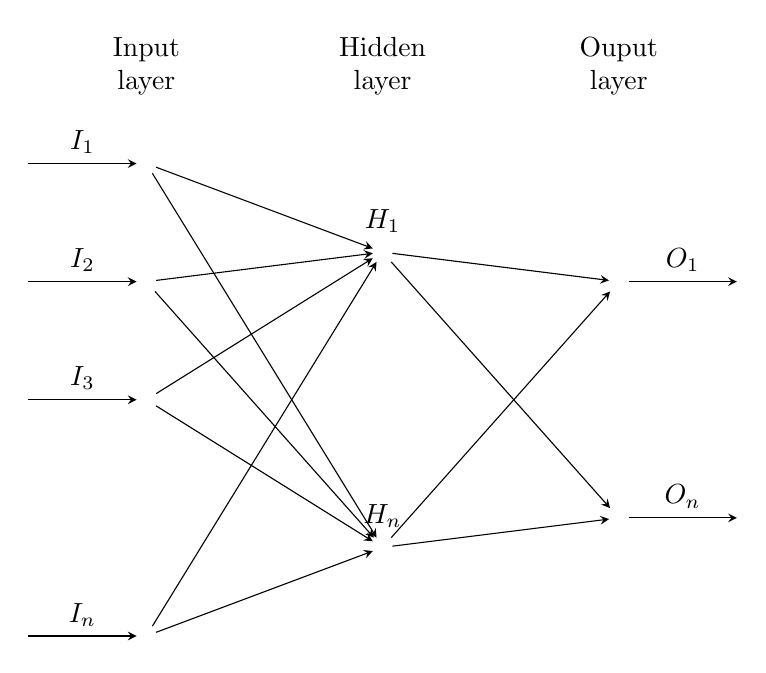
\begin{tikzpicture}[x=1.5cm, y=1.5cm, >=stealth]
	
	\foreach \m/\l [count=\y] in {1,2,3,missing,4}
	\node [every neuron/.try, neuron \m/.try] (input-\m) at (0,2.5-\y) {};
	
	\foreach \m [count=\y] in {1,missing,2}
	\node [every neuron/.try, neuron \m/.try ] (hidden-\m) at (2,2-\y*1.25) {};
	
	\foreach \m [count=\y] in {1,missing,2}
	\node [every neuron/.try, neuron \m/.try ] (output-\m) at (4,1.5-\y) {};
	
	\foreach \l [count=\i] in {1,2,3,n}
	\draw [<-] (input-\i) -- ++(-1,0)
	node [above, midway] {$I_\l$};
	
	\foreach \l [count=\i] in {1,n}
	\node [above] at (hidden-\i.north) {$H_\l$};
	
	\foreach \l [count=\i] in {1,n}
	\draw [->] (output-\i) -- ++(1,0)
	node [above, midway] {$O_\l$};
	
	\foreach \i in {1,...,4}
	\foreach \j in {1,...,2}
	\draw [->] (input-\i) -- (hidden-\j);
	
	\foreach \i in {1,...,2}
	\foreach \j in {1,...,2}
	\draw [->] (hidden-\i) -- (output-\j);
	
	\foreach \l [count=\x from 0] in {Input, Hidden, Ouput}
	\node [align=center, above] at (\x*2,2) {\l \\ layer};
	
	\end{tikzpicture}
\end{minipage}


\subsection{Acoustic Modelling using TDNNs.} 